\documentclass{standalone}
\usepackage{amsfonts,amsmath,amssymb}
\usepackage[slovene]{babel}
\usepackage[utf8]{inputenc}
\usepackage[T1]{fontenc}
  
\usepackage{tikz, verbatim}
\usepackage{pgfplots}
\usetikzlibrary{arrows.meta, calc, positioning, automata}

\begin{document}

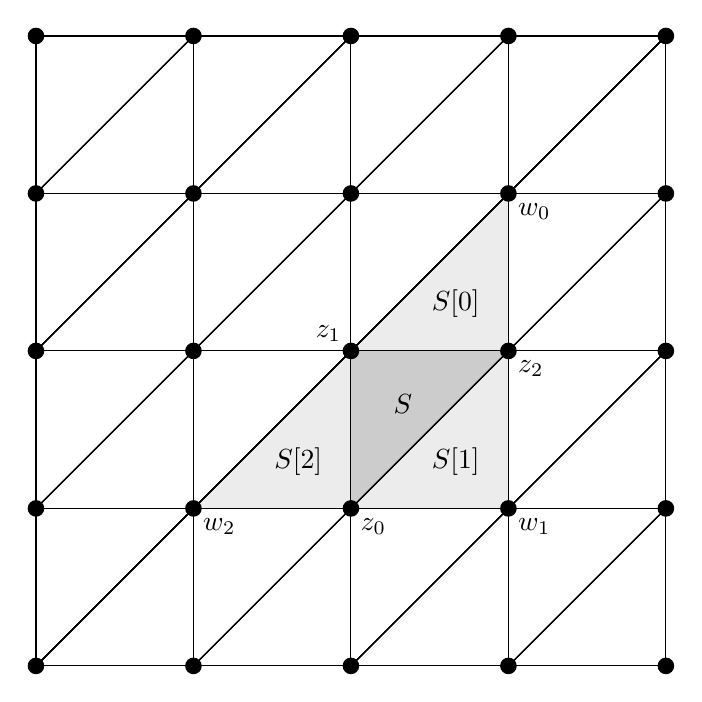
\begin{tikzpicture}
	\fill[fill=gray!40] (4, 2)--(6, 4)--(4, 4);
	\fill[fill=gray!15] (4, 2)--(6, 2)--(6, 4);
	\fill[fill=gray!15] (2, 2)--(4, 2)--(4, 4);
	\fill[fill=gray!15] (4, 4)--(6, 4)--(6, 6);
		
	\foreach \x in {0,2,4,6, 8}
	{   \foreach \y in {0,2,4,6, 8}
	    {  \fill (\x,\y) circle (3pt);
	       \draw (0, \y ) -- (8, \y );
	       \draw (\x ,0) -- (\x ,8);
	       \draw ( 0 , \x) -- ( 8 - \x ,8);
	       \draw ( \x , 0) -- ( 8 ,8 - \x );
	    }
	}	
	
	%\draw (-0.4, 4) node {$C_1^-$};
	%\draw (8.4, 4) node {$C_1^+$};
	%\draw (4, -0.4) node {$C_2^-$};
	%\draw (4, 8.4) node {$C_2^+$};	
	\draw (4, 2) node[below right] {$z_0$};		
	\draw (4, 4) node[above left] {$z_1$};	
	\draw (6, 4) node[below right] {$z_2$};	
	\draw (6, 6) node[below right] {$w_0$};	
	\draw (6, 2) node[below right] {$w_1$};
	\draw (2, 2) node[below right] {$w_2$};	
	\draw (4.66, 3.33) node {$S$};	
	\draw (5.33, 4.6) node {$S[0]$};	
	\draw (5.33, 2.6) node {$S[1]$};	
	\draw (3.33, 2.6) node {$S[2]$};		
	
\end{tikzpicture}
	
\end{document}